\chapter{Methods \& Protocols}

In this chapter, I introduce the main modelling approach and different ideas tested out in this work.

\section{Modelling concept}

\subsection{Model type}

The main model concept is the use of a 2D \acrfull{cnn} to provide 3D segmentation masks, trained on point annotated data.
Out-of-the-box pre-trained 2D networks are available, with weights pre-trained on enormous public datasets\footnote{\label{footnote:Imagenet}For example, weights trained on the ImageNet dataset. 
This dataset consists of \todo[inline]{xxx} images of xxx categories.}.
An alternative approach would be to use 3D networks. This is a logic choice for volumetric data, with the obvious advantage that the 3D convolution layers naturally take into account the structure of the data.
One could argue that using 2D networks deprives the network of important \textit{context} information in the direction perpendicular to the slice it is analysing (I try to meet this issue in section \ref{section:twoDplus} on page \pageref{section:twoDplus}). 

There are also advantages to choosing 2D networks over 3D networks:
\begin{enumerate}
    \item Since the number of parameters (weights) to train scales exponentially with the kernel dimension, the number of parameters to train is considerably higher for a 3D \acrshort{cnn} compared to a corresponding 2D \acrshort{cnn}.
    \item The academic community has been investigating 2D \acrlong{cnn}s for a longer time. The networks can be initialized with weights pretrained on very large and diverse datasets (see remark \ref{footnote:Imagenet} on ImageNet). 
    These datasets indeed do not contain the specific classes, nor the specific datatype investigated in this project. 
    The different convolution layers have proven however to extract useful general features that allow the network to distinguish a very wide range of categories. 
    These features have proven to be sufficiently general to be applicable to new machine vision applications. This practice is called transfer learning \todo{references}.
    \item Although consecutive slices are obviously strongly correlated, one has more data\footnote{There are more slices than volume segments in 1 image volume.} to train the networks. Certainly when considered in proportion to the number of weights to be trained.
\end{enumerate}

\subsection{Model training approach}

An approach used often in weakly supervised learning is the generation of \textit{ersatz} full mask labels.
In this project, I intended to use this approach too.

A scan volume can be sliced along 3 different axis: the transverse axis, the coronal axis and the sagittal axis. 
This means that 3 different models can be trained with the available point annotated data. 
Each of these 3 networks will have different context elements to segment the sliced images on.
The resulting segmentation volumes\footnote{The segmentation results of a stack of 2D slices can be combined to form a 3D segmentation volume.} of these three networks can then be combined to obtain a final segmentation volume.
This final segmentation mask, which should be as least as good as the best of the 3 individual model results, can then be used as \textit{ersatz} masks to train a final \textit{fully supervised} network. 

\begin{SCfigure}[][htb]
    \centering
    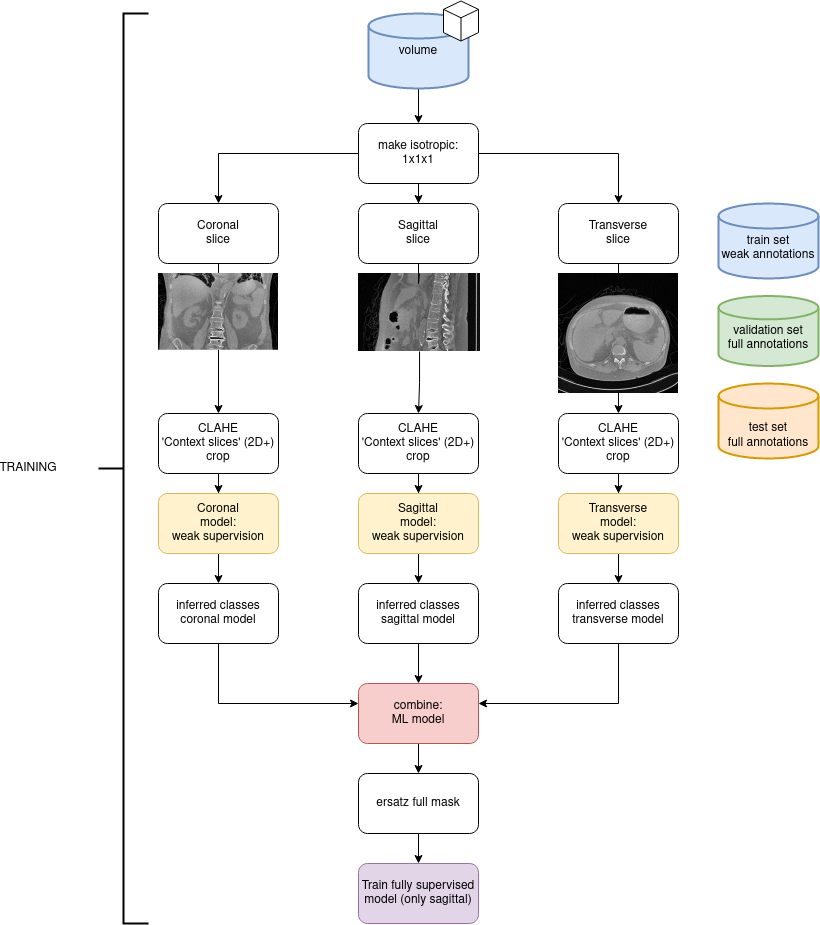
\includegraphics[width=.85\textwidth]{/home/thesis/images/Training_concept.png}
    \caption{\label{fig:model_training_concept}Illustration of the model training approach. 
    This is based on the conbination of 3 different models based on different volume slices.}
\end{SCfigure}

When the segmentation masks of a new, unknown volume need to be inferred, only this final model needs to be evaluated.

\begin{SCfigure}[][htb]
    \centering
    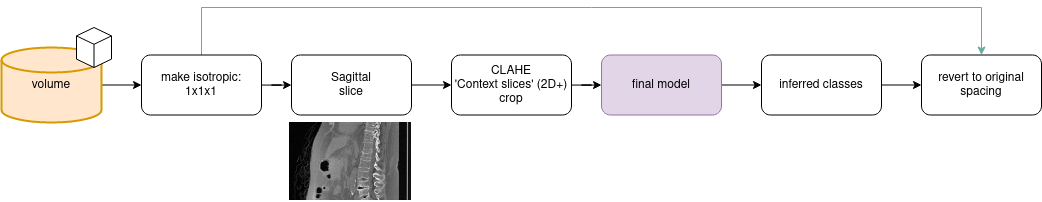
\includegraphics[width=.95\textwidth]{/home/thesis/images/Inference_concept.png}
    \caption{Inference step. Only one model needs to be evaluated in this step, the model that is trianed in the final step of the training procedure illustrated in figure \ref{fig:model_training_concept}.}
\end{SCfigure}
\FloatBarrier
\section{Hyperparameter overview}

Building the different models for the procedure illustrated in figure \ref{fig:model_training_concept} requires to make a number of choices.
In this section, these components are introduced.

\subsection{Network types\label{sec:network_types}}

Three different \acrlong{cnn} architectures were tested for this project:
\begin{description}
    \item[the VGG16 network: ] classic, added some upscore layers.
    \item[The RESNET50 network:] skip connections
    \item[The U-Net network: ] good performance for some biological problems
\end{description}

All of these networks function based on the \textit{encoder - decoder} principle.
\todo{add more insights on the principle}

\begin{SCfigure}[][htb]
    \centering
    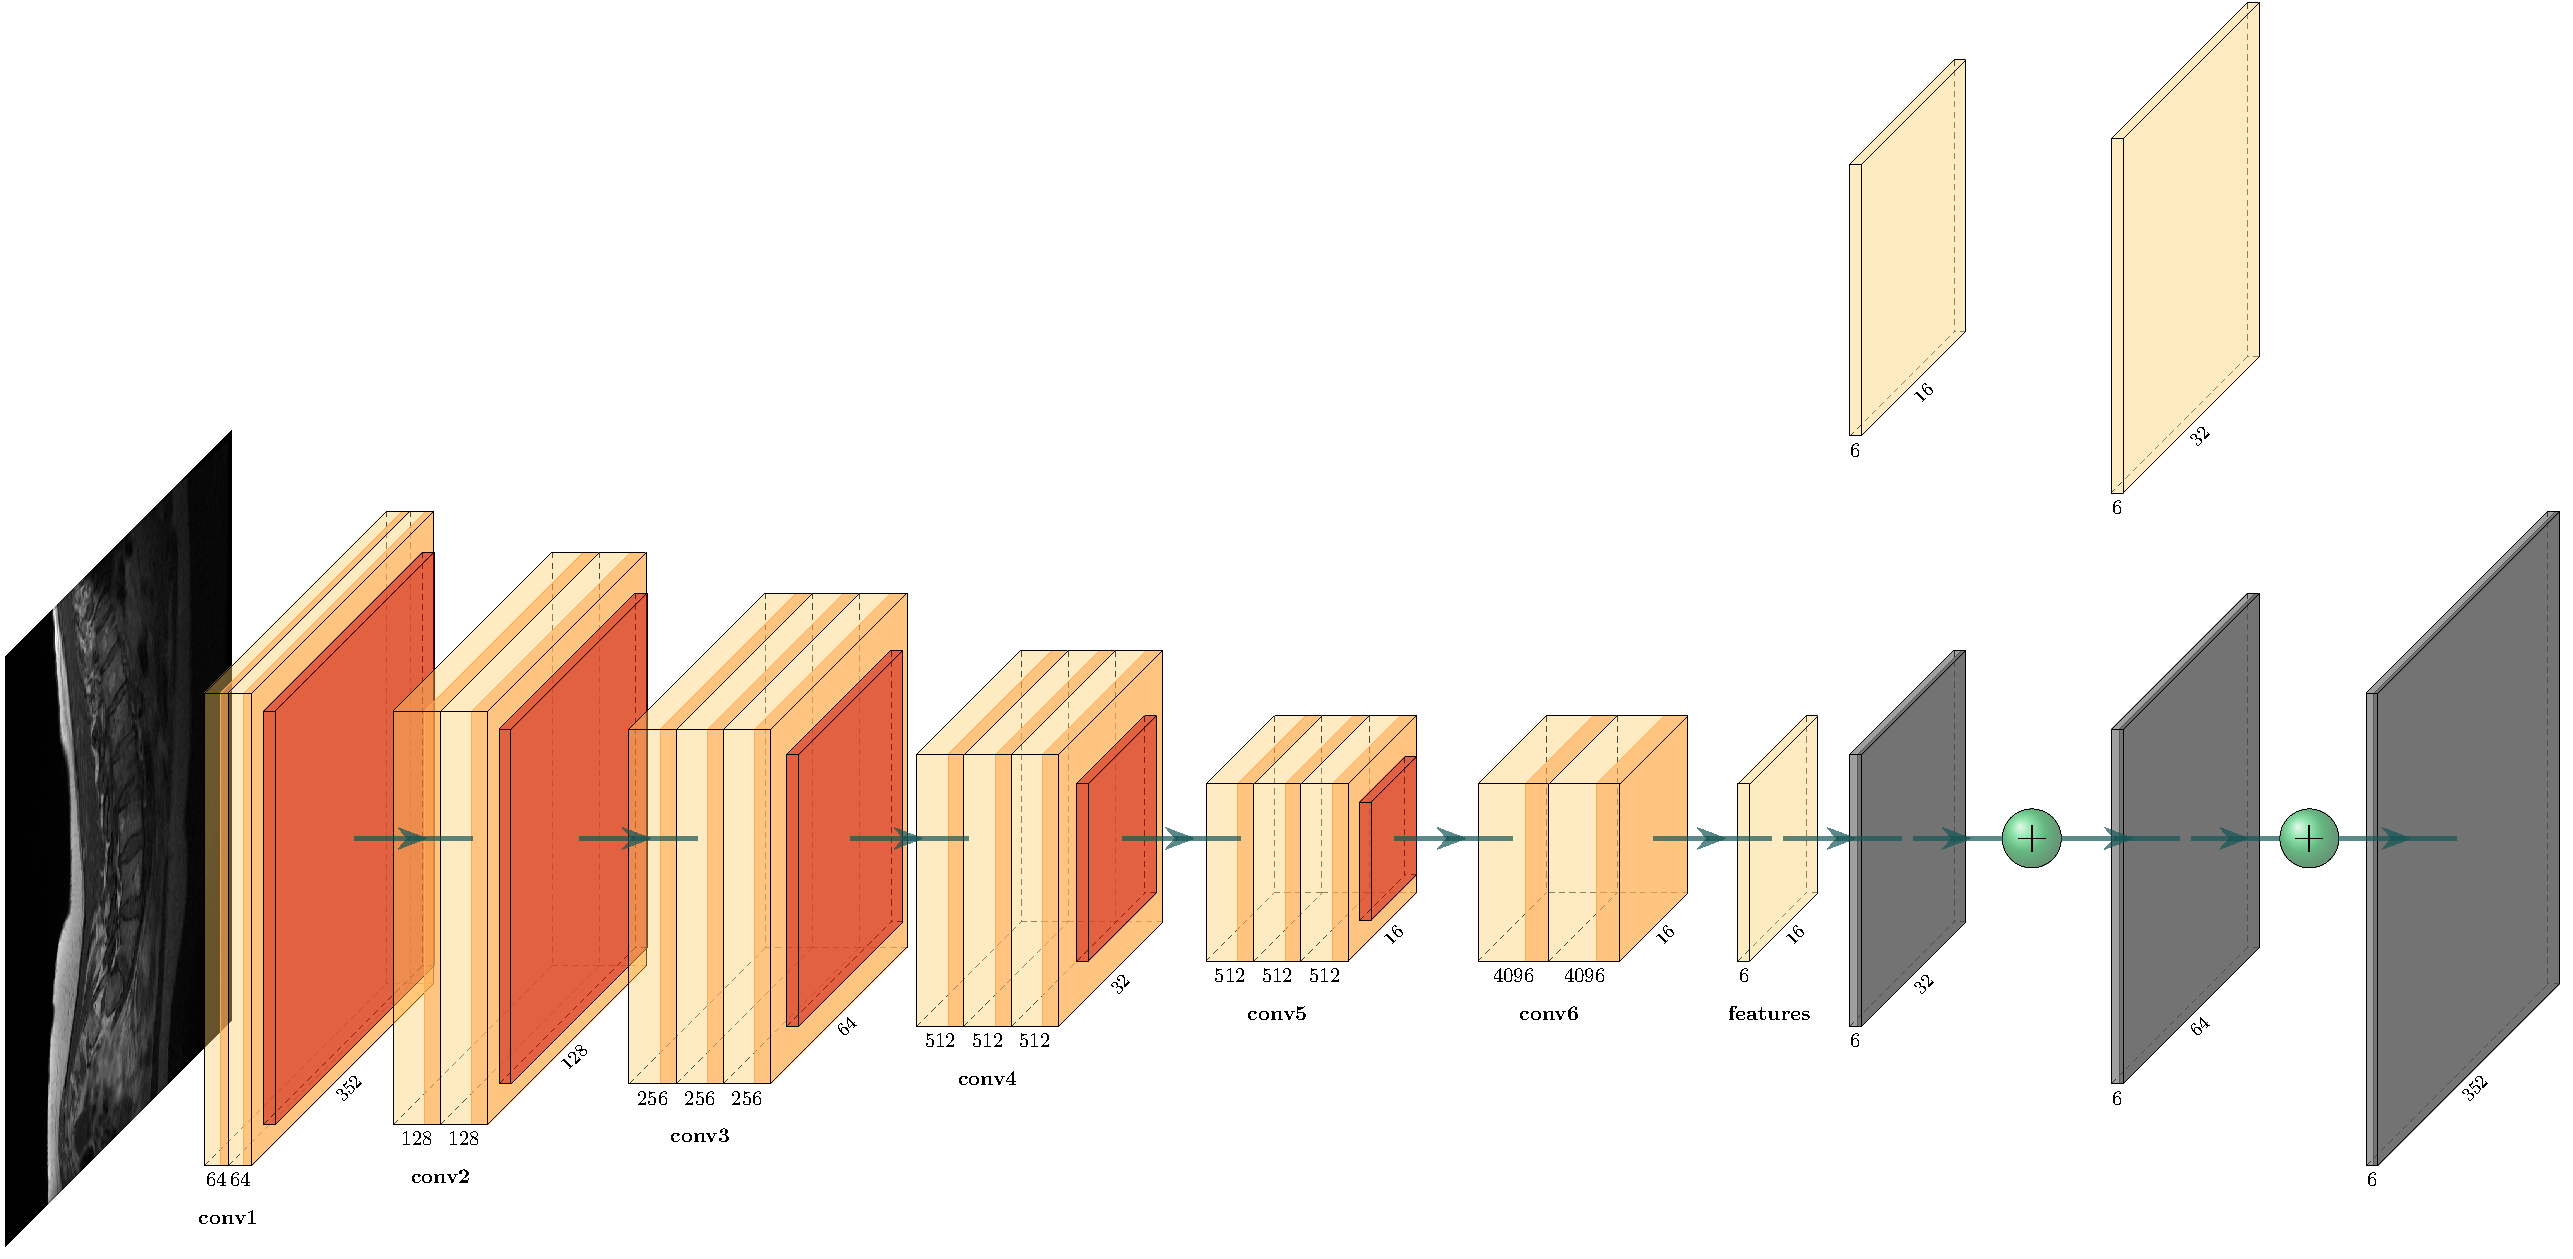
\includegraphics[width=.95\textwidth]{vgg16_upscore.pdf}
    \caption{VGG16 based network}
\end{SCfigure}

\begin{SCfigure}[][htb]
    \centering
    \includegraphics[width=.95\textwidth]{unet.pdf}
    \caption{Unet based network}
\end{SCfigure}

\subsection{2D+ approach and \textit{context slices}\label{section:twoDplus}}

As discussed in section \ref{sec:network_types}, all used networks have a 3 channel\footnote{The networks were originally designed for \textit{RGB}-images with a red, a green and a blue channel.}, 
352$\times$352 pixel input. 
The input images for the network only have 1 channel component. 
The other two channels were used to pass \textit{context} information to the network in the form of the neighboring slices of the slice under investigation.
This combines an essentially 2D approach with a third dimensional element in the form of the extra information of the parallel slices. Thus, this is called the $2D+$ approach.


The hyperparameter to be set $k$ is the index offset for the context slices.
When evaluating slice with index $n$ the slices with indices $\left[n-k; n+k\right]$ are passed as context slices
\footnote{For the edge cases ($n<k$ or $n+k>$ image dimension) when these slices do not exist, slice $n$ is passed as context slice.}.


Several values for $k$ are tested. When $k=0$, no extra slices are taken. The same slice is just entered in all 3 network channels. When $k=1$, the indices directly next to the investigated slices are taken.
Due to the isotropic resampling (see section \ref{sec:resampling}), these slices are physically at 1 mm distance of the center slice. When $k=5$, the slices at $5 mm$ distance from the center slice are used.

\section{Loss functions\label{sec:LossFunctions}}
\par{
    Construction of a machine learning model requires evaluating the model, comparing the result of this evaluation with the desired output and taking steps to make the observed output resemble the desired output better.
    In other words, to train a model, the optimizer will minimize the loss function.
    To use the gradient descent algorithm, this loss function needs to be differentiable.
}
\par{
    Several loss components will be discussed below, both unsupervised and supervised loss functions.
    A supervised loss function component considers the difference between the network prediction and a known (weak) label.
    An unsupervised loss function component considers characteristics of the network output itself. No labels are used in calculating an unsupervised loss component.
    The desirable characteristics that are enforced by the unsupervised loss functions can be part of the \textit{priors}, the knowledge on the problem one has beforehand
    \footnote{To be able to work with weaker, less informative labels, one needs to enter more prior knowledge into the problem}. 
}
In order to make the notation in this section clearer, table \ref{tab:loss_notations} list the notations used in the loss function components.
\begin{SCtable}[\sidecaptionrelwidth][h]
 
    \begin{tabular}{ l l } 
     \hline
     \hline
     Symbol & meaning \\
     \hline 
    $n$                 & Number of problem classes \\
    $X_i$               & Slice $i$ and corresponding context slices   \\ 
    $\vec{p}$           & A pixel position in slice $i$ \\
    $\mathcal{K}$       & Set of outcome classes: $\mathcal{K} = [0, 1, \dots, n-1]$ \\
    $\mathcal{Y}_i$     & set of labels for slice $i$, $\mathcal{Y}_i(\vec{p}) \in \mathcal{K}$  \\
    $\mathcal{I}_i$     & set of pixel positions for which a label is available \\
    $f_\theta(X_i)=z_i$ & model output (logits) for $X_i$ with weights $\theta$. $\vec{z_i(\vec{p})}\in \mathbb{R}^n$ \\
    $\sigma(z_i(\vec{p}))$   & softmax result for $\vec{z_i(\vec{p})}$ ($\in \mathbb{R}^n$ and $\forall k\in \mathcal{K} 0\leq\sigma_k\leq1$) \\
    $w_k$ & A weigth that can be attributed to class $k \in \mathcal{K}$ \\
     \hline
     \hline
    \end{tabular}
    \caption{List of symbols used in the loss functions\label{tab:loss_notations}}

\end{SCtable}
\par{
    In this project, $n=6$ for the coronal and sagittal slice models and $n=2$ for the transverse slice models. 
    Label $\mathcal{Y}_i(\vec{p})=0$ indicates the background class and the lubar vertebrae $L_m$ are indicated with $\mathcal{Y}_i(\vec{p})=m$ ($m\in[1,2,3,4,5]$).
    In the fully supervised case, $\mathcal{I}_i$ spans the complete slice $i$. In the weakly supervised case, there are only a handful of positions $\vec{p}$ for which a label exists.
}
The softmax function $\sigma$ is related to the sigmoid function $\mathbf{S}$. It is defined as:

\begin{eqnarray}
    \sigma_k(z) &=& \frac{\exp(z_k)}{\sum_{m\in\mathcal{K}} \exp(z_m)} \\
    \mathbf{S}(x) &=& \left[ 1+ exp(-x) \right]^{-1} \\ &=& \frac{exp(x)}{exp(x) + 1} 
\end{eqnarray}

The final training loss is given by:
\begin{equation}
    \mathcal{L} = \mathcal{L}_P + \mathcal{L}_E + \mathcal{L}_C + \mathcal{L}_S
\end{equation}
The different loss components are detailed below.

\subsection{Supervised loss functions}

\subsubsection{cross entropy loss\label{sec:crossentropy} \& Point loss}
To compare the network output with the labels, first, the (weighted) cross entropy loss is used\footnote{The weight is optional. One can decide $\forall i\in\mathcal{K}: w_i=1$}.

\begin{equation}
\mathcal{L}_P(X_i) = -\sum_{\vec{p} \in \mathcal{I}_i} w_{\mathcal{Y}_i(\vec{p})}.\log\left[\sigma_{\mathcal{Y}_i(\vec{p})}\left(\vec{z_i(\vec{p})}\right)\right]
\label{eq:LP}
\end{equation}

This loss term is minimized when the network output $z_i(\vec{p})[k]$ with $k=\mathcal{Y}_i(\vec{p})$ the class label for $\vec{p}$ is maximal while the other logits for this position are minimal.
In the fully supervised case, this loss function is called the cross entropy loss. 
When training a model with point supervision, this is only one of multiple loss components. 
In the case of point supervised data, $\mathcal{I}_i$ only consists of a handful of points.
This loss component is in this case called the point loss component $\mathcal{L}_P$.

\subsubsection{Prior extend loss}
The second supervised loss function used is the \textit{prior extend} loss.
This loss function describes the prior knowledge that the dimensions of a vertebra are limited. 
Based on \cite{Alam2014}, the maximal extent of a human lumbar vertebrae was set to be $r=110mm$.
This means that a point label $\mathcal{Y}_i(\vec{p})=m: m\in[1,2,3,4,5]$ indicating that $\vec{p}$ is a point in vertebra $L_m$, also means that all points outside of a cicle with radius $r$ cannot be points of $L_m$.
\marginpar{
        % This file was created by tikzplotlib v0.9.8.
\begin{tikzpicture}

\begin{axis}[
height=5cm,
tick align=outside,
width=5cm,
x grid style={white!69.0196078431373!black},
xmin=-0.5, xmax=349.5,
xtick pos=both,
xtick style={color=black},
y dir=reverse,
y grid style={white!69.0196078431373!black},
ymin=-0.5, ymax=349.5,
ytick pos=left,
ytick style={color=black}
]
\addplot graphics [includegraphics cmd=\pgfimage,xmin=-0.5, xmax=349.5, ymin=349.5, ymax=-0.5] {images/prior_extend-000.png};
\addplot [draw=black, fill=black, mark=*, only marks, scatter]
table{%
x  y
120 80
100 35
};
\end{axis}

\end{tikzpicture}

        \captionof{figure}{Illustration of the prior extend mask for annotation points at [120, 80] and [100, 34]. In the grey area, $\mathbf{m} = 0$.}
        \label{fig:prior_extent}
    }
First, $n-1$ (in this case 5) distance masks are created\footnote{1 label is background, for which there is no prior extend.}, 
representing the maximal\footnote{Maximal distance, because there can be mulitple such labels.} distance (Euclidian norm) of each location $\vec{q}$ from the label $\mathcal{Y}_i(\vec{p})=k$ furthest away from $\vec{q}$.
Then $\mathbf{d}$ is converted to a semi-mask:
\begin{eqnarray}
    \mathbf{d}_k(\vec{q}) &=& \max_{\vec{p}:\mathcal{Y}_i(\vec{p})=k}||\vec{q} - \vec{p}||\\
    \mathbf{m}_k(\vec{q}) &=& \mathbf{I}\left( (-\mathbf{d}(\vec{q}) + r) > 0 \right)
\end{eqnarray}
Now, $\mathbf{m}$ is 1 for positions closer than distance $r$ from the points, and it is 0 for positions far from labels with value $k$.
Where $\mathbf{m}_k=0$, the model output should not indicate output class $k$. Where $\mathbf{m}_k=1$, the output class is unknown\footnote{Only channel $k$ is concerned, since one only knows what class these points do not belong to, there is not more information about the other classes.}.

The loss function is the binary cross-entropy between $\mathbf{m}_k$ and the sigmoid of the k$^{th}$ channel of the logits $z_i$ with weight vector $\{1, 0\}$.

\begin{equation}
    \mathcal{L}_E(X_i) = \sum_{k\in\mathcal{K}}\sum_{\vec{q}\in X_i}  (1-\mathbf{m}_k(\vec{q})) \log(\mathbf{S}(z_i(\vec{q})_k)) 
\end{equation}

%\footnote{
%    The cross-entropy loss is easier to interpret when one considers the binary case ($n=2$) over $N$ datapoints with true value $t_i \in \left\{0;1\right\}$ and softmax probability $0 \leq p_i \leq 1$ ($i\in \{0;..;N-1\}$) is defined as 
%\begin{equation}
%    \mathcal{L} = -\frac{1}{N} \left(  
%        \sum^{N-1}_{i=0} \left(
%            t_i log(p_i) + (1 - t_i) log( 1 - p_i )
%        \right)
%     \right)
%\end{equation}}


\subsection{Unsupervised loss functions}

\subsubsection{Transformation consistency loss}
The first unsupervised loss function is the unsupervised consistency loss \todo{cite Laradji}. 
The idea behind this loss is that the model output should be consistent for geometric transformations of the input.
A set of geometrical transformations $T=\left\{ t_1, t_2, \dots, t_n \right\}$ is defined. 
Then the consistency loss function $\mathcal{L}_C$ is defined as
\footnote{This function evaluates the difference between the transformation of the model output $t_k\left[f_\theta(X_i)\right]$ and the model output for the transformed input $f_\theta\left( t_k[X_i] \right)$.}
\begin{equation}
    \mathcal{L}_C(X_i) = \sum_{p \in \mathcal{P}_i} \left| t_k\left[f_\theta(X_i)\right]_p - f_\theta\left( t_k[X_i] \right)_p  \right|  
\end{equation}.

In this project, two transformations are combined: rotations of $[90^{\circ}, 180^{\circ}, 270^{\circ}]$ and the horizontal flip.
Each time the loss is called, 1 transformation $t$ is randomly selected from the list, and the transformation consistency loss is calculated using this transformation.

\subsubsection{Separation loss}
As mentioned when discussing the cross-entropy loss in §\ref{sec:crossentropy}, this loss encourages the model to output the correct label and to decrease the output values for the other labels.
As discussed, the right label is often not know for most of the locations in a weakly supervised problem.
Apart from a limited number of points, there is no such incentive for weakly supervised networks.
For this reason, the separation loss $\mathcal{L}_S$ is introduced.
This loss component consists of the negative sum of the absolute difference of the class segmentation masks\footnote{$z_i[m]$ denotes the $m^{th}$ model output channel.}:
\begin{equation}
    \mathcal{L}_S(X_i) = - \sum_{\vec{p}} \sum_{m\in \mathcal{K}} \sum_{n \in \mathcal{K}, n>m} \mathbf{S}(z_i[m]) - \mathbf{S}(z_i[n])
\end{equation}

This loss component thus provides an incentive to the network to make a decision, even in areas where few annotation points are available.
\section{Metrics}
\par{Metrics are used to evaluate and compare \acrlong{ml} models.
This text focuses on the important metrics used for multi-class classification problems.
\marginpar{
% Please add the following required packages to your document preamble:
% \usepackage{multirow}
%\begin{table}[]
    \begin{tabular}{cllll}
    \hline
    \multicolumn{1}{l}{}                &                        & \multicolumn{3}{l}{\textbf{Actual class}}           \\
    \multicolumn{1}{l}{}                &                        & $C_0$   & $C_1$   & $C_2$                        \\ \cline{3-5} 
    \multirow{3}{*}{\rotatebox[origin=c]{90}{\parbox[c]{1cm}{\centering \textbf{Predicted class}}}}   & \multicolumn{1}{l|}{$C_0$} & $a_{0,0}$ & $a_{0,1}$ & \multicolumn{1}{l|}{$a_{0,2}$} \\
                                        & \multicolumn{1}{l|}{$C_1$} & $a_{1,0}$ & $a_{1,1}$  & \multicolumn{1}{l|}{$a_{1,2}$ } \\
                                        & \multicolumn{1}{l|}{$C_2$} & $a_{2,0}$  & $a_{2,1}$  & \multicolumn{1}{l|}{$a_{2,2}$ } \\ \hline
    \end{tabular}
    %\end{table}

    \captionof{table}{Illustration of confusion matrix with 3 classes.}
    \label{tab:confusionMatrix}
    }}
\par{
    The example in table \ref{tab:confusionMatrix} will be used to introduce the different metrics.
    Table \ref{tab:confusionMatrix} illustrates a confusion matrix for a model for a problem with 3 classes ($C_j:j\in \{1;2;3\}$). 
    A model predicts the class for all observations in the set.
    The confusion matrix allows comparing these predictions against the true class\footnote{The true class is the label for this observation.}.
    $a_{0,0}$, $a_{1,1}$, $a_{2,2}$ are the correctly labelled observations. 
The predicted class corresponds to the actual class.
This is not necessarily the case for all observations. For example, $a_{1,2}$ observations with true class $C_2$ the model predicted to belong to class $C_1$.
In general, $a_{i,j}$ is the number of observations for which the model predicted $C_i$ and for which the label is $C_j$.
Based on the confusion matrix, 3 metrics can be calculated: the model \textit{precision}, the \textit{recall} and the \textit{F-score}.
}
\subsection{Class imbalance\label{sec:class_imbalance}}
\par{
    To construct an appropriate set of metrics to use for a problem, the class distribution of the dataset\footnote{
        One hopes that through a good data collection strategy, the dataset represents the population on which we ultimately want to infer.
        } needs to be taken into account.
    Imagine, for example, that one aims to segment pixels in a set of pictures where 95\% of the pixels is of the \textit{background} class and 5\% of the pixels is of the class to be segmented.
    A model can now quickly obtain 95\% accuracy by predicting every pixel as \textit{background}. This is not a metric suitable for the problem.
}
\par{
    For an evaluation metric to be useful, it has to avoid the kind this kind of pitfall.
    In this work, I investigate a problem where most of the image under investigation is \textit{background}. 
    There is about 1 pixel of each of the lumbar vertebra classes for 500 background pixels.
    The different performance metrics for the different classes are weighted with the inverse of their relative occurrence to evaluate the model's performance correctly.
}
\subsection{Precision}
\par{
    The \textbf{precision}\footnote{the precision is also called the \textit{positive predictive value}.}, for class $i$,\footnote{
        Note that for binary classifiers (reject a null-hypothesis $H_0$ or do not reject $H_0$) the metrics for the positive class are understood to be the classifier metrics. 
        One will traditionally report the classifier precision as $\frac{TP}{TP+FP}$ without calculating the precision for the negative class where $H_0$ is not rejected.
        The binary confusion matrix clarifies the meaning of TP (True Positive) and FP (False Positive).
        \begin{tabular}{clll}
            \multicolumn{1}{l}{}                &                        & \multicolumn{2}{l}{\textbf{Actual}}           \\
            \multicolumn{1}{l}{}                &                        & $H_0$   & $\neg H_0$                         \\ \cline{3-4} 
            \multirow{2}{*}{\textbf{Pred.}}   & \multicolumn{1}{l|}{$H_0$} & $TN$ & \multicolumn{1}{l|}{$FN$} \\
                                                & \multicolumn{1}{l|}{$\neg H_0$} & $FP$  & \multicolumn{1}{l|}{$TP$ } \\ \hline
            \end{tabular}.\\
    } is the proportion of true labels $C_i$ out of all observations predicted to be $C_i$. 
    For example, the precision for class 1 in table \ref{tab:confusionMatrix} is:
    \begin{equation}
        \text{Precision}_1 = \frac{a_{1,1}}{a_{1,0} + a_{1,1} + a_{1, 2}} \tag{Precision$_1$ in table \ref{tab:confusionMatrix}}
    \end{equation}.
    In general, the Precision$_i$ for class $C_i$ in a problem with $k$ classes is given by equation \ref{eq:precision_i}.
    \begin{eqnarray}
        \text{Precision}_i &=& \mathcal{P} \left( label = C_i \mid prediction = C_i \right) \\
        &=& \frac{a_{i, i}}{\sum_{j=0}^{k-1} a_{i, j}} \label{eq:precision_i}
    \end{eqnarray}
}
\par{
    One can thus calculate the precision metric for each class. 
    To calculate a precision metric for the complete multi-label classifier
    , one can either aggregate the class precisions by taking the arithmetic mean (this is called the Macro-precision: $Precision_M$) or by taking the weighted mean (this is called the weighted-mean precision: $Precision_w$).
    To take the weighted mean, each precision term $Precision_i$ is weighted by the number of observations with label $C_i$. 
    \begin{eqnarray}
        \text{Precision}_M &=& \frac{\sum_{i=0}^{k-1} \text{Precision}_i}{k}  \label{eq:macro_metric}\\
        \text{Precision}_w &=& \frac{\sum_{i=0}^{k-1} \left[ \text{Precision}_i \sum_{j=0}^{k-1} a_{j,i} \right] }{\sum_{i=0}^{k-1} \sum_{j=0}^{k-1} a_{i,j} }  \label{eq:weighted_metric}
    \end{eqnarray}
}




\subsubsection{Recall}
\par{
    The \textbf{recall}\footnote{The recall is also called the \textit{sensitivity}.} is the numer of correctly predicted $C_i$ observations out of the total number of $C_i$ observations.
    For example, the recall for class 1 in table \ref{tab:confusionMatrix} is:
    \begin{equation}
        \text{Recall}_1 = \frac{a_{1,1}}{a_{0,1} + a_{1,1} + a_{2, 1}} \tag{Recall$_1$ in table \ref{tab:confusionMatrix}}
    \end{equation}.
    The general expression for recall$_i$ is equation \ref{eq:recall_i}.
    \begin{eqnarray}
        \text{recall}_i &=& \mathcal{P} \left( prediction = C_i \mid label = C_i \right) \\
        &=& \frac{a_{i, i}}{\sum_{j=0}^{k-1} a_{j, i}} \label{eq:recall_i}
    \end{eqnarray}
    The weighted-mean recall and macro-recall are defined in the same way as the multi-label precision metrics, see equation \ref{eq:macro_metric} and equation \ref{eq:weighted_metric}.
}




\subsection{Dice score\label{sec:dice}}
\par{
    The objective is, of course, to build a model with both high precision and a high recall.
    There is often a trade-off to be made. 
    Increasing the recall tends to reduce the precision
    \footnote{To increase recall$_i$, you need to encourage the model to predict $C_i$. Unfortunately, this increases the probability that an observation is wrongly classified as $C_i$, thus decreasing precison$_i$.}.
    One needs to find a balance between both.
}
\newpage
\par{It is useful to combine both metrics in a single new metric: the \textbf{F1-score}\footnote{The F1-score is also called the Dice-score}. This is accomplished by taking the harmonic mean
\footnote{The harmonic mean assures that F1 will always be between the values of precision and recall, but it will be closer to the lowest value. If, for example, $recall=0$ and $precision=1$, then $F1=0$.} of precision and recall.
\begin{equation}
    \text{Dice}_i = 2 . \frac{precision_i \times recall_i }{precision_i + recall_i }
\end{equation}
}
\par{
    Calculation this for Dice$_1$ in the example shows the dice score can also be described as double the intersection 
    between the points predicted as $C_1$ and the points with true label $C_1$ devided by the sum of the number of points predicted as $C_1$ and the number of points with true label $C_1$.
    \begin{equation}
        \text{Dice}_1 = \frac{2.a_{1,1}}{a_{0,1} + 2.a_{1,1} + a_{2, 1} + a_{1,0} + a_{1,2}} \tag{Dice$_1$ in table \ref{tab:confusionMatrix}}
    \end{equation}
}
\par{
    Now, there are several options for aggregation in the multi-class case:
    There are two macro F1-scores in use:
    \begin{description}
        \item[macro F1-score]: Calculate the F1-score for each class and take the arithmatic mean of the $k$ class F1-scores. As discussed in §\ref{sec:class_imbalance}, for inbalanced problems, a weighted mean can help to more acurately describe the model quality.
        \item[macro F1*-score]: Calculate the class precision and recall scores. From these class precision and recall scores, calculate the macro precision and macro recall score. 
        The macro F1*-score is given by\\ $F1_M^*=2 . \frac{precision_M \times recall_M }{precision_M + recall_M }$
        \item[weighted F1-score]: Calculate the F1 score for all classes and calculated the weighted average as is done in equation \ref{eq:weighted_metric} to calculate the weighted precision.
    \end{description}
}
In this work, the weighted F1-score or weighted Dice score is used to evaluate the experiment results in part \ref{part:results} starting at page \pageref{part:results}.
For clarity, the expression defining $\text{Dice}_w$ is iterated below\footnote{Remark that $\sum_{j=0}^{k-1} a_{j,i}$ corresponds to all true labels that are equal to $i$.}:
\begin{equation}
    \text{Dice}_w = \frac{\sum_{i=0}^{k-1} \left[ \text{Dice}_i \sum_{j=0}^{k-1} a_{j,i} \right] }{\sum_{i=0}^{k-1} \sum_{j=0}^{k-1} a_{i,j} } \label{eq:weighted_dice}
\end{equation}

\subsection{Intersection over Union}

The \textbf{\acrfull{iou}}\footnote{The \acrshort{iou} is also known as the Jaccard score.} is closely related to the Dice score.
IoU is the area of overlap between the predicted segmentation and the ground truth divided by the area of union between the predicted segmentation and the ground truth.
In the given example, the \acrshort{iou} score for $C_1$ is:
\begin{equation}
    \text{IoU}_1 = \frac{a_{1,1}}{a_{0,1}+a_{1,1}+a_{2,1}+a_{1,0}+a_{1,2}} \tag{IoU$_1$ in the table \ref{tab:confusionMatrix}}
\end{equation}

In general, the class specific \acrfull{iou} for class $C_i$ is given by:
\begin{equation}
    \text{IoU}_i = \frac{a_{i,i}}{\sum_{j=0}^{k-1} a_{i, j} + \sum_{j=0}^{k-1} a_{j,i} - a_{i,i}} 
\end{equation}

Again, a macro IoU score can be calculated by taking the arithmetic mean of the class IoU scores.

\subsubsection{Classifier accuracy}

Finally, the classifier accuracy is defined as the proportion of the observations that is correcly classified:
\begin{equation}
    \text{accuracy} = \frac{a_{0,0} + a_{1,1} + a_{2,2}}{\sum_{i=0}^{2} \sum_{j=0}^{2} a_{i,j}   } \tag{table \ref{tab:confusionMatrix} classifier accuracy}
\end{equation}

In general, the classifier accuracy is defined by 
\begin{equation}
    \text{accuracy} = \frac{\sum_{i=1}^{k-1}a_{i,i}}{\sum_{i=0}^{k-1} \sum_{=0}^{k-1} a_{i,j}   } 
\end{equation}




\section{Investigation strategy}

\begin{SCfigure}[][htb]
    \centering
    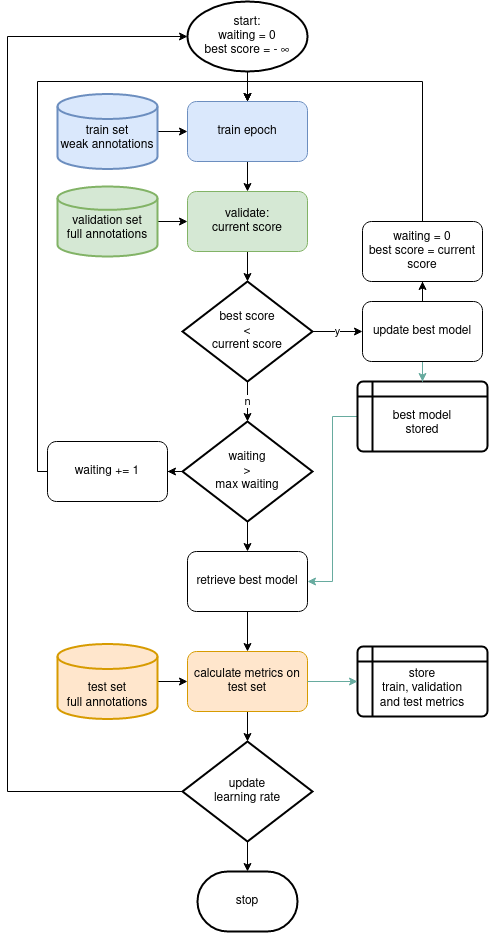
\includegraphics[width=.95\textwidth]{/home/thesis/images/model_optimization.png}
    \caption{training}
\end{SCfigure}

\section{Fully supervised model}



\section{Fully supervised model}

\subsection{Model}

Lessmann, discussed in xxx.
The specific implementation is based on github repo xxx.

\subsection{Data}

Discussion on approach for using the datasets I have with the Lessmann model.
How to preprocess the different datasets?
What data augmentation steps used?

\subsection{Hyperparameters}

Hyperparameters for model and training from \cite{Lessmann2018}

\section{Weakly supervised model}

The weakly supervised model is based on \gls{wise}, introduced in \cite{Laradji2020}.
This network consists of a Localization branch, based on \gls{lc-fcn} and an Embedding branch.

\subsection{Model}

Model is based on \gls{wise}.

The Localization network \gls{lc-fcn} is a \acrfull{fcn} trained with a \acrfull{lc}.
this \acrshort{lc} constists of 4 sublosses: image level loss, point level loss, split level loss, split level loss.d

\subsection{Data}

2D model -> volumes are sliced.
Discussion of this procedure

\subsection{Hyperparameters}

\begin{SCfigure}[][htb]
    \centering
    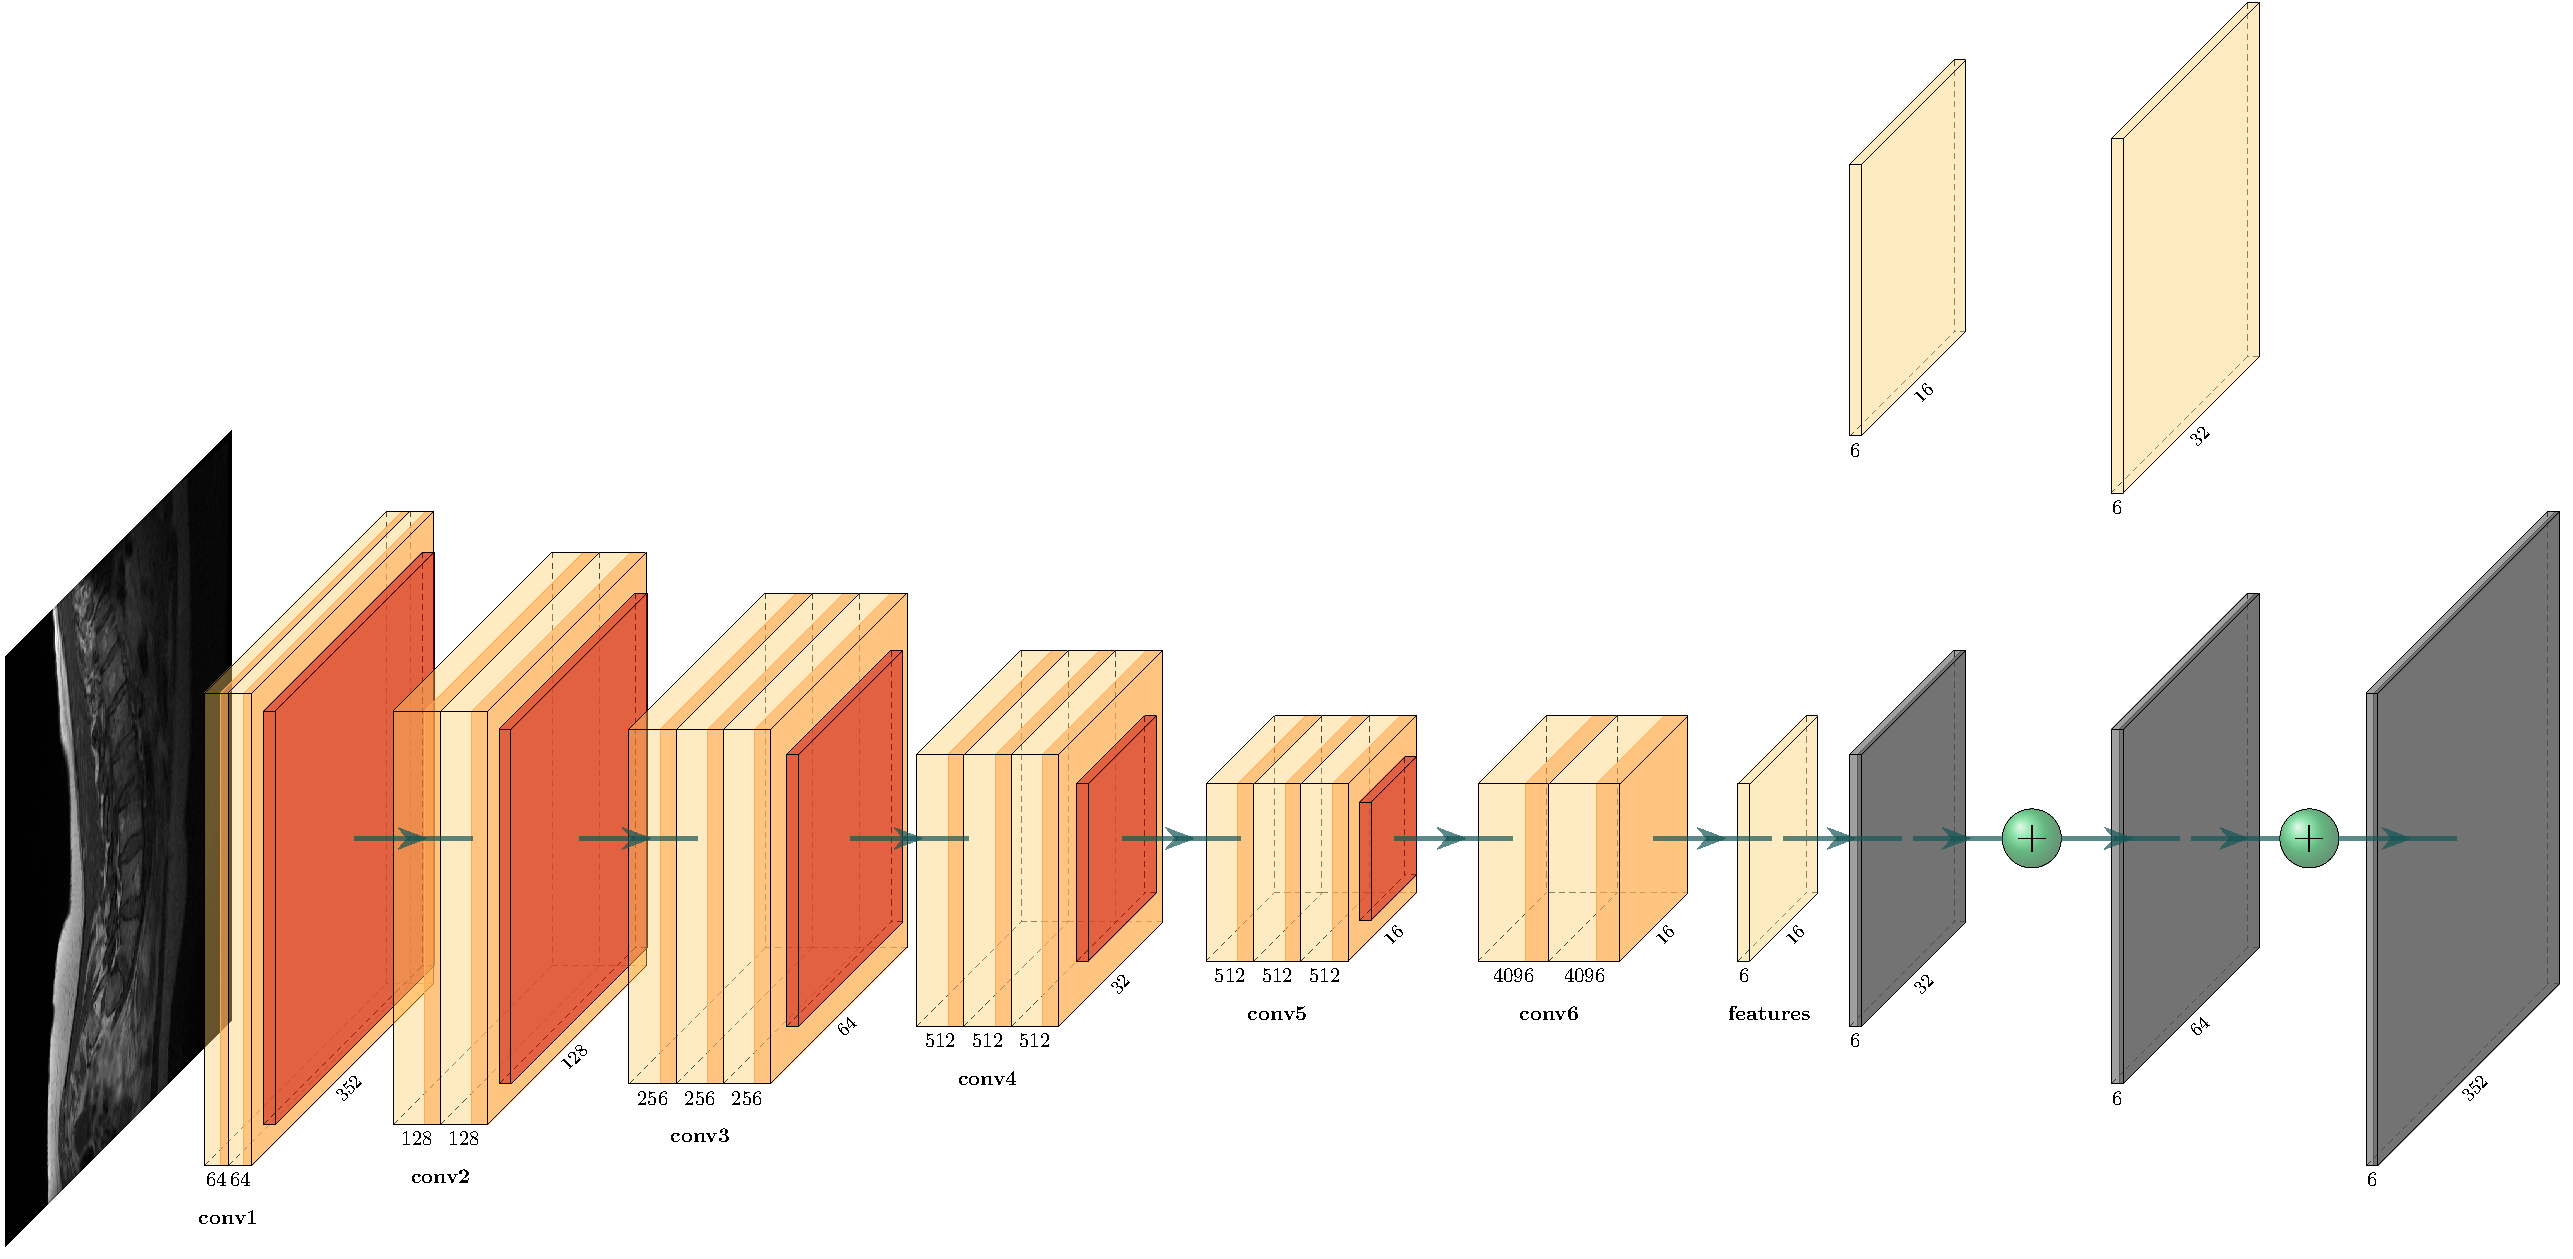
\includegraphics[width=.95\textwidth]{vgg16_upscore.pdf}
    \caption{VGG16 based network}
\end{SCfigure}

\begin{SCfigure}[][htb]
    \centering
    \includegraphics[width=.95\textwidth]{unet.pdf}
    \caption{Unet based network}
\end{SCfigure}

